% Capitolo 4

\chapter{Un prototipo di servizio federato}
\label{Capitolo4}
\lhead{Capitolo 4. \emph{Un prototipo di servizio federato}}

L'uso delle tecnologie digitali offre nuove possibilità per
l'insegnamento. Molte comunità, afferenti alla RM, hanno iniziato la
produzione di materiale pedagogico audio-visuale, che con l'aiuto
della rete, potrebbe contribuire ad arricchire i programmi educativi
pubblici spesso carenti e poco integrati con la cultura quilombola. Il
\emph{Núcleo de Pesquisa e Desenvolvimento Digital (NPDD)}\footnote{Il
  \emph{Núcleo de Pesquisa e Desenvolvimento Digital (NPDD)} della RM
  ricerca e sviluppa tecnologie digitali per la comunicazione, la
  produzione di energie rinnovabili e sostenibili, e il miglioramento
  delle condizioni di vita in simbiosi con l'ambiente. Maggiori
  informazioni su \url{http://wiki.mocambos.net/wiki/NPDD}.}, nucleo
di ricerca e sviluppo digitale della RM, con il progetto \emph{Tambor
  e Comunicação}\footnote{Il progetto \emph{Tambor e Comunicação} é un
  tentativo di fortificare la rete di comunicazione digitale per le
  necessità delle comunità. Vedi
  \url{http://wiki.mocambos.net/wiki/Projeto_Tambor_e_Comunicacao}.},
ha proposto la ricerca e sviluppo di una soluzione per la
pubblicazione e diffusione in rete di immagini, audio e video di
interesse comune e spesso prodotti nelle stesse comunità.

\section{Sistema di pubblicazione e diffusione di contenuti
  multimediali}
Il sistema sviluppato prevede l'installazione di un portale sul server
locale delle comunità su cui è possibile pubblicare contenuti
multimediali, sfruttando l'alta velocità della rete locale. Il sistema
si prende cura di diffondere i contenuti, etichettati come di
interesse comune, verso i server delle altre comunità (vedi figura
\ref{fig:SchemaServer_ReteMocambos}). Il prototipo sviluppato cerca di
risolvere le limitazioni di banda della rete rispettando la specifica
di requisiti.

\begin{figure}[htbp]
  \centering
  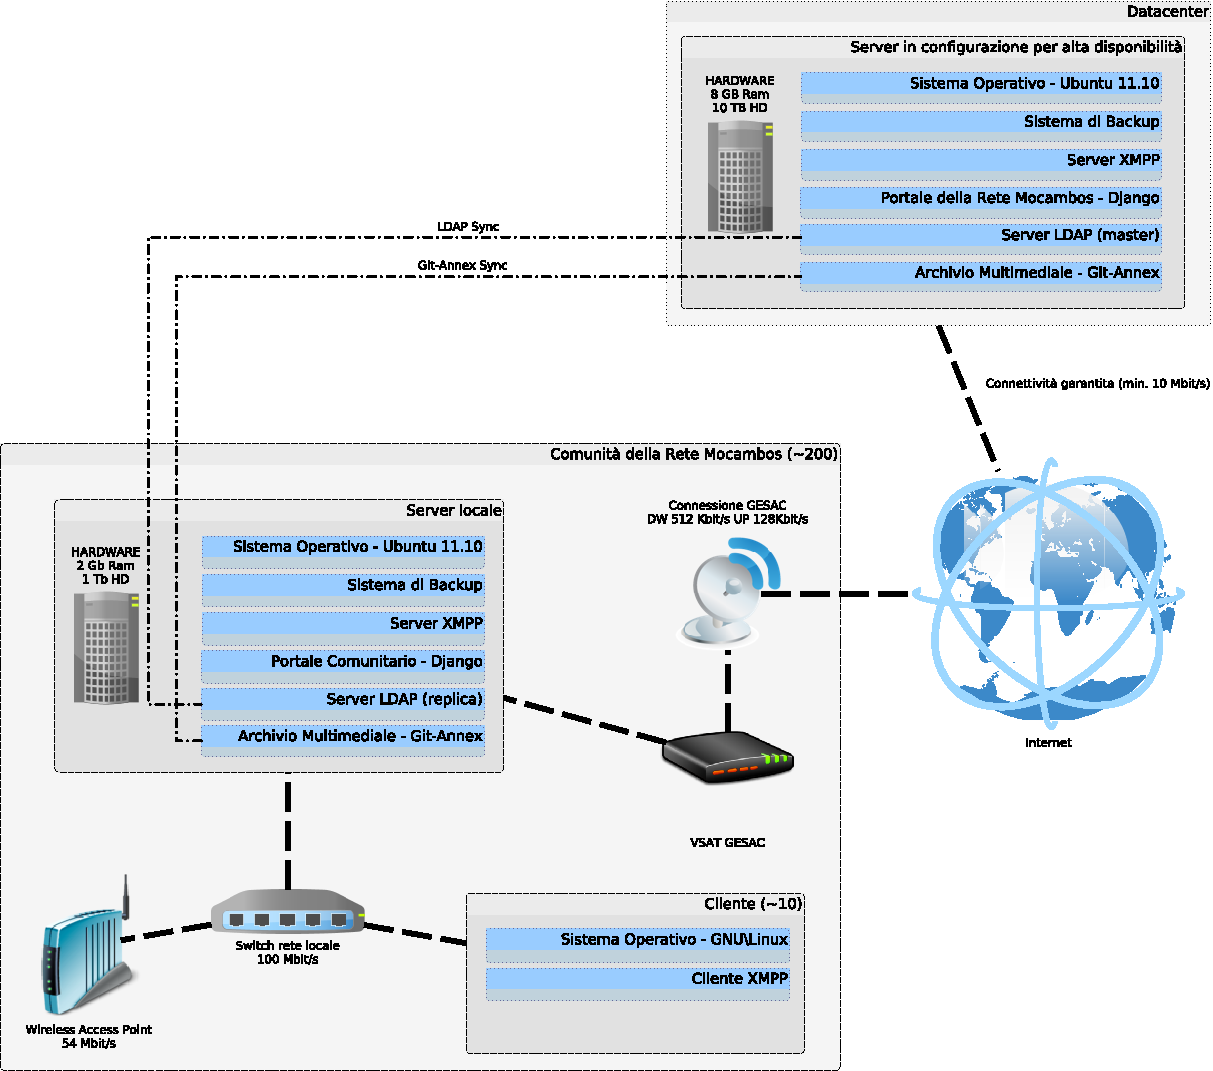
\includegraphics[width=\textwidth]{./Figure/SchemaServer_ReteMocambos-crop.pdf}
  \rule{35em}{0.5pt}
  \caption[Schema dell'infrastruttura della RM]{Schema dell'infrastruttura della RM.}
  \label{fig:SchemaServer_ReteMocambos}
\end{figure}

\section{Archivio multimediale}
L'archivio locale della comunità è un \emph{repository git-annex} che
viene gestito tramite il portale comunitario, sia per la pubblicazione
che per la visualizzazione dei contenuti. L'accesso diretto ai dati è
comunque garantito essendo i dati salvati in chiaro sul disco.

\subsection{git-annex}
\emph{git-annex}\footnote{\emph{git-annex} è un programma libero
  disponibile su \url{http://git-annex.branchable.com}.}
permette la gestione di file con \emph{git}, senza la necessità di
aggiungere il file dentro \emph{git}. Anche se può sembrare
paradossale, è utile quando si ha a che fare con file molto grandi che
\emph{git} attualmente non può gestire facilmente per limitazioni
dovute a memoria, tempo o spazio nel disco.

Anche senza mantenere traccia del contenuto del file, avere la 
possibilità di gestire i file con \emph{git}, di spostarli e cancellarli su un
albero di cartelle versionato, con uso di \emph{branches} e di cloni
distribuiti, sono tutti buoni motivi per usare \emph{git}. E i file allegati
(da cui il nome \emph{git-annex}) possono coesistere nello stesso repository
\emph{git} con i file regolarmente versionati.

\emph{git-annex} trasforma i file allegati in \emph{link}
simbolici, che vengono normalmente versionati da \emph{git}. 

Il contenuto dei file viene mantenuto da \emph{git-annex} in un
archivio chiave/valore distribuito che corrisponde ai cloni di un
dato \emph{repository git}. Praticamente \emph{git-annex} memorizza il
contenuto del file in una sotto-cartella di \verb|.git/annex/|.

La prima volta che un file viene aggiunto a \emph{git-annex}, viene
calcolata una chiave, normalmente facendo un \emph{hash} del suo
contenuto. \emph{git-annex} tuttavia supporta diversi \emph{backend}
che possono produrre vari tipi di chiavi. Il file che viene aggiunto a
\emph{git} non è altro che un \emph{link} simbolico alla chiave
memorizzata in \verb|.git/annex/|. Se il contenuto del file viene
modificato, viene prodotta un'altra chiave, e il \emph{link} viene
cambiato.

Il contenuto del file può essere trasferito da un \emph{repository}
all'altro da \emph{git-annex}, che inoltre mantiene traccia di chi
contiene cosa, permettendo ad esempio di creare una mappa delle copie
disponibili e impostare il numero di copie minime. Queste informazioni
vengono mantenute su un \emph{branch} separato, chiamato
``\emph{git-annex}'', e le operazioni di sincronizzazione non sono
altro che \emph{push} e \emph{pull} tra i vari \emph{repository}.

\emph{git-annex} supporta:
\begin{itemize}
\item localizzazione delle copie (\emph{location tracking})
\item scaricamento selettivo dei contenuti
\item gestione della fiducia dei \emph{repository}
\item gestione del numero di repliche minimo 
\item vari \emph{backend} per le chiavi (SHA, WORM)
\item vari \emph{backend} per i contenuti/valori (bup, rsync, web, S3)
\end{itemize}

\section{Portale Comunitario}
Il portale locale deve dare accesso ai principali servizi locali della
comunità. Per lo sviluppo è stato scelto l'uso di un framework basato
su python, \emph{Django}, che consente un'integrazione flessibile e
avanzata con altri sistemi grazie alle numerose librerie disponibili
quale, ad esempio, quella per l'autenticazione LDAP.

Per gestire l'archivio multimediale \emph{git-annex} sono stati
sviluppati due moduli per \emph{Django}, che definiscono il modello
dei dati e si prendono cura di aggiungere i contenuti sul
\emph{repository} eseguendo le operazioni di \emph{commit},
\emph{push} e \emph{pull}. 

\begin{figure}[htbp]
  \centering
  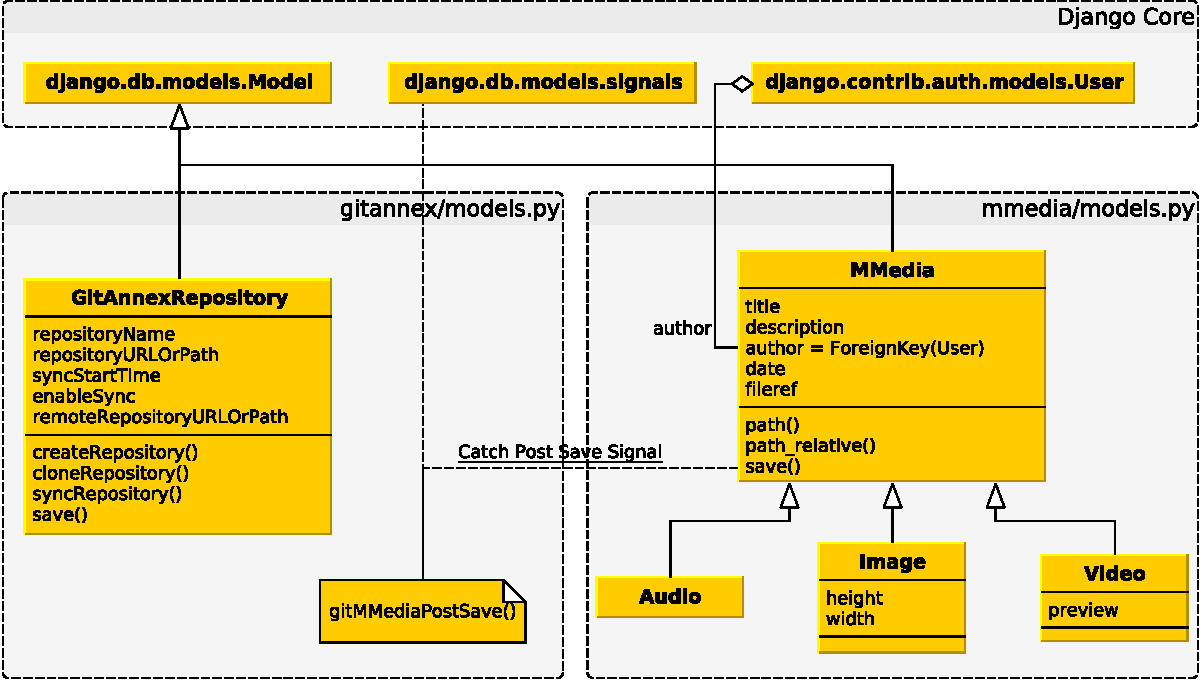
\includegraphics[width=\textwidth]{./Figure/UML_Schema_Django-crop.pdf}
  \rule{35em}{0.5pt}
  \caption[Schema UML dei moduli django]{Schema UML dei moduli django.}
  \label{fig:SchemaUMLDjango}
\end{figure}

\subsection{Django}
\emph{Django} è un framework per lo sviluppo rapido di applicazioni web.
